\section{Introduction}
Large Language Models are multimodal architectures, such as CLIP.

\textbf{Multimodal architectures}: refers to computational models designed to process and integrate data from multiple modalities, or types of input. For example, these architectures can combine text, images, audio, and other forms of data to create a more comprehensive understanding or prediction.   


In this chapter we will focus on Image Encoder in a multimodal setup. Using this settings, we aim to create robust networks capable of consuming different input types to learn a more robust visual representations. 


\section{Image Encoder}

In Figure \ref{fig:LLM-Image-encoder}, we have outlined all the approaches available for training an image encoder. So far, we have covered 2 out of the 4 sections: \textbf{Supervised Learning} (CNN) and \textbf{Contrastive Language-Image Pre-training} (CLIP). The remaining topics are \textbf{Image-Only (Non-) Contrastive Learning} and \textbf{Masked Image Modeling}.

All these methods share the same goal: to build a robust model capable of learning strong visual data representations. For many years, supervised learning was the state-of-the-art approach. However, with the invention of BERT, the focus shifted to \textbf{Masked Image Modeling}. Subsequently, the community transitioned to \textbf{Image-Only (Non-) Contrastive Learning}, exemplified by methods like DINO. Currently, CLIP has become the state-of-the-art.

\begin{figure}[H]
    \centering
    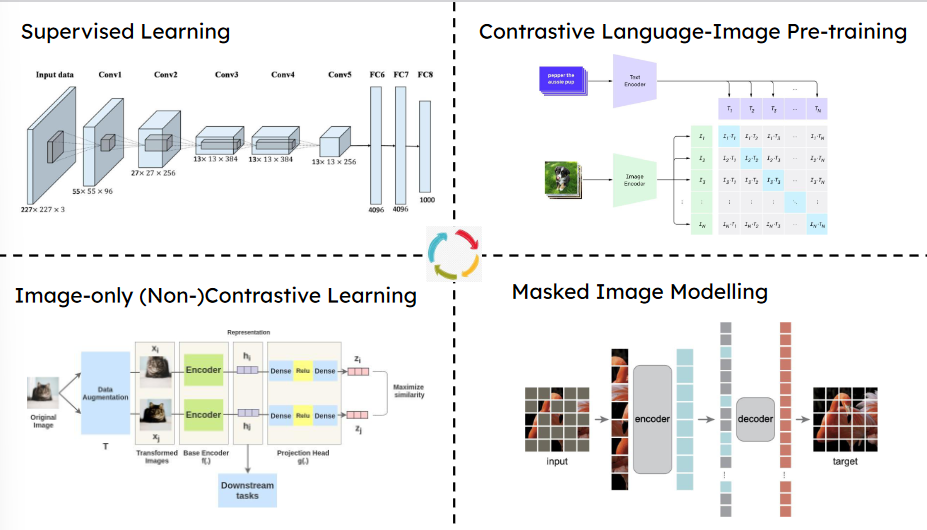
\includegraphics[width=1\linewidth]{tikz/LLM Image Encoder.png}
    \caption{LLM Image encoder classes}
    \label{fig:LLM-Image-encoder}
\end{figure}

\subsection{Supervised Learning}

The goal is to develop a powerful visual encoder by learning a mapping from image space to a discrete label space associated with visual concepts. However, this approach faces a bottleneck due to the high costs of human annotation. Consequently, researchers created large private datasets such as JFT-300M, JFT-3B, and IG-3.6B. Additionally, they found that noisy labels can regularize the network, resulting in better and more universal image embeddings.

\begin{figure}[H]
    \centering
    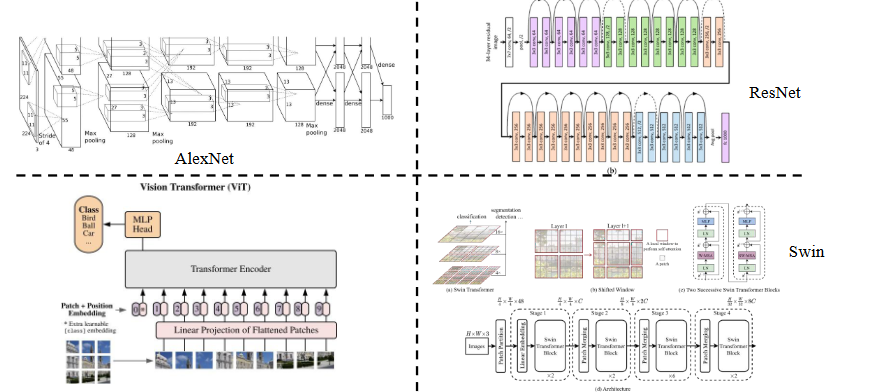
\includegraphics[width=1\linewidth]{Image Encoder supervised.png}
    \caption{Examples of Image Encoder Supervised Learning}
    \label{fig:Image-encoder-supervised}
\end{figure}

\subsection{Image-only (Non-) Contrastive Learning}

The first alternative to the previous class that emerged was \textbf{SimCLR}, a Simple Framework for Contrastive Learning of Visual Representations.


\begin{figure}[H]
    \centering
    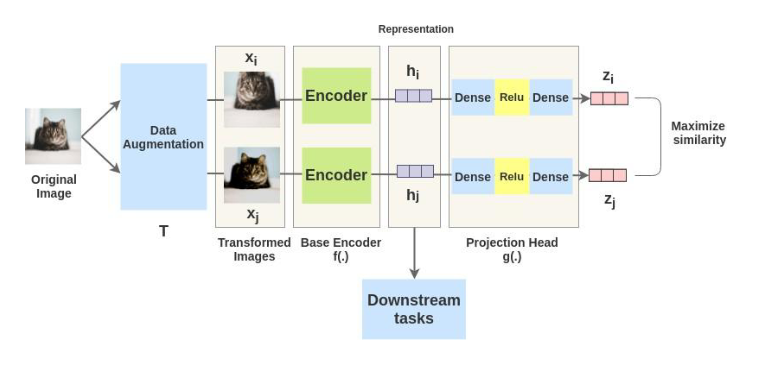
\includegraphics[width=0.75\linewidth]{tikz/SimCLR.png}
    \caption{SimCLR architecture}
    \label{fig:enter-label}
\end{figure}

Here's how it works: given an image, two separate data augmentations are applied. Each augmented image is then processed by a base encoder $f()$, producing corresponding fixed latent representation vectors. These vectors are subsequently passed through a projection head $g()$, which maps them into another latent space, resulting in $ z_i$ and $ z_j $. Each projection head module consists of a sequence of dense fully connected layers, ReLU activations, and a final dense layer. The vectors $z_i $ and $z_j$ are used in the \textbf{contrastive loss} function, specifically \textbf{InfoNCE}, to perform the training. The goal is to maximize the agreement between the augmentations, determining whether they originate from the same image or not.


The InfoNCE loss function for SimCLR is defined as:

$$
\mathcal{L}^{(i,j)}_{\text{InfoNCE}} = - \log \frac{\exp(\text{sim}(\mathbf{z}_i, \mathbf{z}_j)/\tau)}{\sum_{k=1}^{2N} \mathbb{1}_{[k \neq i]} \exp(\text{sim}(\mathbf{z}_i, \mathbf{z}_k)/\tau)}
$$

where:
\begin{itemize}
    \item $\text{sim}(\mathbf{z}_i, \mathbf{z}_j)$ is the cosine similarity between the representations $\mathbf{z}_i$ and $\mathbf{z}_j$.

    \item $\tau$ is a temperature parameter that controls the scale of the distribution.
    \item $\mathbb{1}_{[k \neq i]}$ is an indicator function that equals 1 if $k \neq i$ and 0 otherwise.
    \item $N$ is the number of positive pairs (i.e., augmented images).
\end{itemize}

In practice, the InfoNCE loss maximizes the similarity between representations of augmented image pairs (positive pairs) and minimizes the similarity between representations of unrelated images (negative pairs) within the minibatch.

The projection head is discarded for downstream tasks, as the better representations are $ h_i $ and $h_j$ instead of $z_i$ and $z_j$. Although this model is competitive with supervised learning state-of-the-art methods (by using a pre-trained encoder, attaching a fully connected layer, and training it), it requires a large batch size to ensure sufficient negative samples for each class.

Recent research has addressed this issue by reducing the dependency on negative samples. Alternatives include \textbf{asymmetric architectures} (BYOL, SimSiam), \textbf{dimension de-correlation} (Barlow Twins), and \textbf{clustering} (SWaV, DINO). These methods share the principle that the representations of a sample and its transformation should be similar.

\subsubsection{DINO}

DINO (Distillation with No Labels) is a Vision Transformer (ViT) model that employs a self-supervised loss. It is widely recognized for its ability to compute segmentation maps that emerge from the self-attention modules of the transformer.

The architecture utilizes a \textbf{teacher-student} framework with a \textbf{cross-entropy loss}. The student network extracts the parameters of interest. As DINO falls under the clustering approach, the output of the student network is passed through a softmax function to determine if an image belongs to a certain cluster. This produces a probability distribution, enabling training with a \textbf{self-supervised cross-entropy loss}. The teacher network is updated using the exponential moving average (EMA) of the parameters learned by the student network.

To ensure the teacher makes precise predictions for a given class, centering and softmax layers are added. The centering layer subtracts the mean feature, and the output is sharpened by using a low softmax temperature.

The gradient is propagated only through the student network, allowing the use of centering on the teacher model.

\begin{figure}[H]
    \centering
    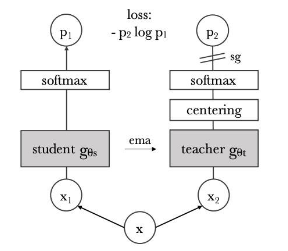
\includegraphics[width=0.75\linewidth]{tikz/DINO.png}
    \caption{An example of DINO}
    \label{fig:DINO}
\end{figure}


\textbf{Clustering tends to address the problem of batch size by learning a powerful visual encoder through a self-supervised loss. Furthermore, aside from normal constrains that ensure that the network's representations will be similar (teacher-student), some extra constrains (centering and softmax) are needed otherwise the feature will collapse. Extra-constrains, loss and architecture change from paper to paper.}




\subsection{Masked image modeling}

In this class of learning, models are learnt to predict a missing part of the input (masked) given other (unmasked) information.

\subsubsection{BEiT}

The model works by taking an image and divide it into patches. Then, some of them are masks and all the patches are flatten into a vector. This vector becomes the input (plus positional embedding) of the \textbf{BEiT encoder}, which is a pre-training of Image Transformers. We then retrieve only the embeddings related to the masked tokens. The choosen embedding are then passed as input to an extra encoder, the \textbf{Masked Image Modelling Head}. This represents what we want to learn at the end. To do this, we employ supervision help.

To facilitate this process, an additional network is employed. Before pre-training, an "image tokenizer" is learned via VQ-VAE/GAN, which tokenizes an image into discrete visual tokens. These visual tokens serve as the supervisor for the encoder. The encoder (\textbf{Masked Image Modeling Head}) can thus be viewed as a form of \textbf{knowledge distillation} \footnote{"Knowledge distillation" is a process where a smaller model (the "student") learns to replicate the behavior of a larger, more complex model (the "teacher"). The student model is trained to match the teacher's outputs, making it more efficient while maintaining similar performance.} between the image tokenizer and the BEiT encoder, with the key difference being that the BEiT encoder only views a portion of the image.

At the end, we use a pre-trained decoder to predict masked visual tokens.

\begin{figure}[H]
    \centering
    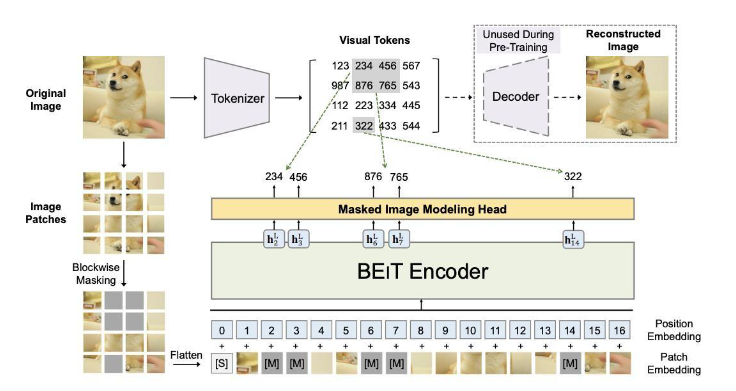
\includegraphics[width=1\linewidth]{tikz/BERT.png}
    \caption{An example of BERT}
    \label{fig:BERT}
\end{figure}

The model works pretty well with fine-tuning rather than pre-training. Of course, one reason realted to this fact is the complexity of the model. Thus, variation have been developed. For example, \textbf{MAE} uses the pixel values as targets instead of the visual tokens. The model is very aggressive in masking patches, as a large random subset of images (0.75) is masked out. Then, the encoder is trained to produce representation of only visible patches. Before the decoder, the masked patches are re-applied with latent representations. The decoder then reconstructs the original image.

\begin{figure}[H]
    \centering
    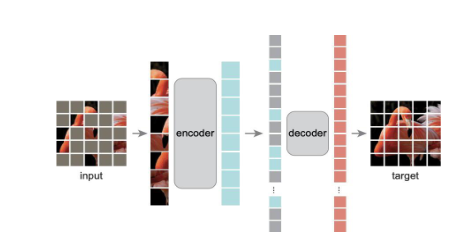
\includegraphics[width=1\linewidth]{tikz/MAE.png}
    \caption{An example of MAE}
    \label{fig:MAE}
\end{figure}

\subsection{Contrastive language-image pre-training}

This type of model is the current SOA. The architecute employes both a visual and text encoder. \textbf{It learns image representations from web-scale noisy text supervision}. The training is made by simple \textbf{contrastive loss}, large-scale pre-training.

Thanks to its special architecture, we are able to perform a new type of downstream task, \textbf{zero-shot image} classification and image-text retrieval. Thus, image classification can be recasted (can be transformed) as a retrieval task via considering the semantics behind label names (security camera example).


\begin{figure}[H]
    \centering
    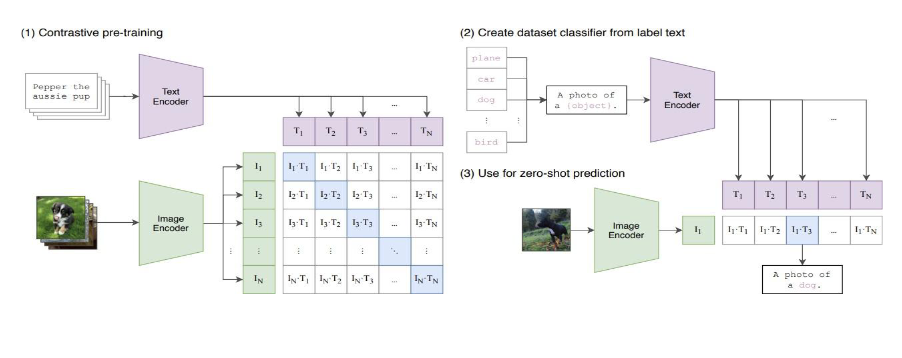
\includegraphics[width=1\linewidth]{tikz/CLIP.png}
    \caption{An example of CLIP}
    \label{fig:CLIP}
\end{figure}

One of the reason why CLIP works is because it is a simple algorithm that scales well. Language provides richer supervision than traditional closed-set labels, offering more comprehensive information. Consequently, CLIP can scale across both \textbf{model and data} dimensions: the model by adjusting the two encoders, and the data by training on billions of image-text pairs. Additionally, batch size is crucial, typically set at 32k, and the model size is significant. Moreover, CLIP enhances open-vocabulary visual recognition capabilities by learning from Internet-scale image-text pairs.

However, CLIP has some limitations: 
\begin{enumerate}
    \item CLIP does not go directly from image to text or viceversa. It just connects the image and text embedding spaces.

    \vspace{5 pt}

    \item CLIP can only address limited use cases such as classification

    \vspace{5 pt}

    \item It crucially lacks the ability to generate language which makes them less suitable to more open-ended tasks such as captioning or visual question answering
\end{enumerate}

How can we improve the model?
Basically, we can make improvements in three macro areas: \textbf{data scaling}, \textbf{model design} and \textbf{objective functions}.

\begin{figure}[H]
    \centering
    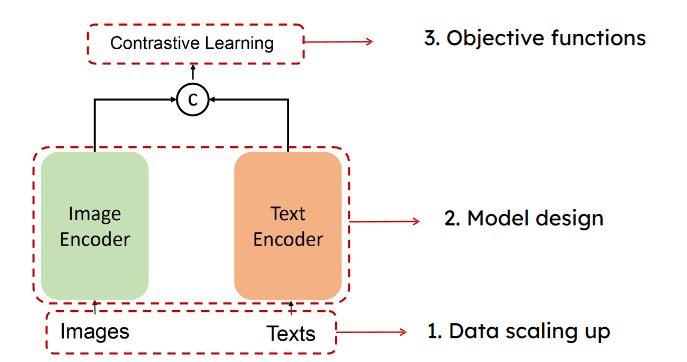
\includegraphics[width=0.75\linewidth]{tikz/CLIP improvements.png}
    \caption{An example of CLIP improvements}
    \label{fig:CLIP-Improvements}
\end{figure}

\subsubsection{Data Scaling up}
This paper used pre-trained open CLIP with LAION-2B across various scales, namely model, data, ecc..

The take home message is that scale matters, but how can we further scale it up? One solution could just be search of the next-generation image-text datasets. However, researchers understood that filtering the data that is feed to the model leads to better results with less dataset size. \textbf{DATA MATTERS!}.

\subsubsection{Model design}
Many improvements can be made both for the visual and language model designs.

\textbf{Image Side}

An example is \textbf{FLIP}, which tried to scale CLIP training (more efficient) via randomly masking out image patches with a high masking ratio. This allows the image encoder to process just the non-masked patches. Thus, during training we still use CLIP loss, but no reconstruction of masked patches is made.

Results showed that this does not hurt performance, but improves training efficiency

\begin{figure}[H]
    \centering
    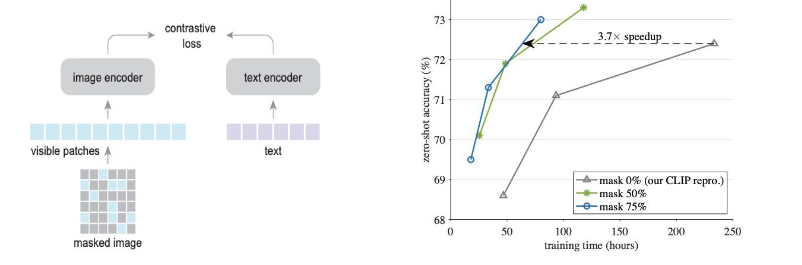
\includegraphics[width=1\linewidth]{tikz/FLIP.png}
    \caption{An example of FLIP}
    \label{fig:FLIP}
\end{figure}

\textbf{Language Side}

Since the classes are very fine-graned, this paper introduces a mechanism to expand the knowledge of the text, \textbf{external knowledge}, in order to provide more information. This can be done very easily as the text encoder can be fed with arbitrary input length (original text + external knowledge).


\begin{figure}[H]
    \centering
    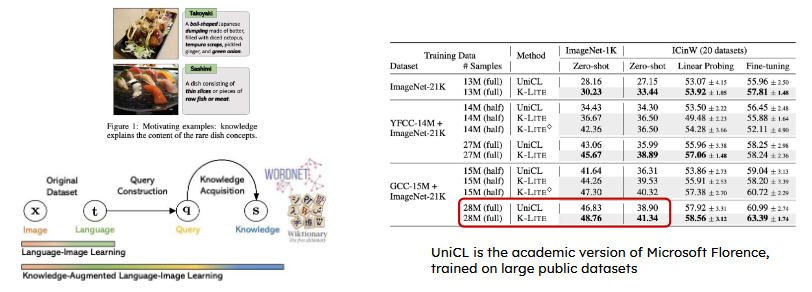
\includegraphics[width=1\linewidth]{tikz/K-Lite.png}
    \caption{An example of K-Lite}
    \label{fig:K-Lite}
\end{figure}

As we can see from the figure above, the \textbf{expanding knowledge} mechanism is executed in two phases: during training, the model is endowed with an ability to read and understand a specific knowledge source (\textbf{query)}. The knowledge is retrieved from an external source such us WordNet (in different levels); during evaluation the knowledge provides an additional information source to enhance model inference.

Results showed that for dataset containing specific images, such us Flowers, the knowledge expention  led to performance improvements as the extra knowledge helped to better discriminate among classes, whereas for dataset like Eurosat it worked poorly becuase the extra-knowlegde retrieved was unrelated to the image. Thus, the closer the retrieved knowledge is to the image, the better performances are reached.


\textbf{Multi Modalities}

In this case, the scale up is made by adding more modalities rather than 2 (like audio, video, ecc...). For example,  \textbf{ImageBind} used one out of 7 modalities employed as anchors (images) and others that will allign to this one key modality (like text, audio, ecc...).  Thus, we link all modalities (7) into a common space. A pre-trained CLIP is used and kept frozen, i.e., learning other modality encoders to align the CLIP embedding space.


\begin{figure}[H]
    \centering
    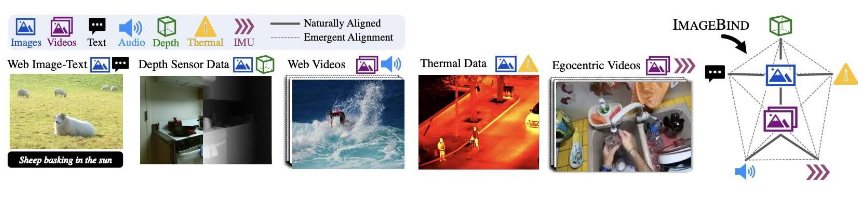
\includegraphics[width=1\linewidth]{tikz/ImageBinf.png}
    \caption{An example of ImageBind}
    \label{fig:ImageBind}
\end{figure}

The model employs pairs of modalities (I,M), where I signifies images and M is another modality, to learn a \textbf{single joint embedding}. Each modality’s embedding is aligned with image embeddings, for instance, text is aligned with images using web data, and IMU data is aligned with video because we do not have an extra-pair for IMU and Image data. The embeddings and encoders are optimized using an \textbf{InfoNCE loss}.

ImageBind has shown an \textbf{emergent behavior}: the model is able to align the two different modalities
(M1,M2) even though it is trained using only the pairs (I,M1) and (I,M2). For instance,
it achieves state-of-the-art zero-shot text-audio classification results without being
exposed to any paired audio-text samples (as most of datasets are paired originally only with images).


\textbf{Interpretability}

Another problem of CLIP is that we do not have any for of interpretability of the embedding space of an image. 
The training procedure aims to learn sparse semantic embeddings that associate each word with a score, effectively mapping images and text to a high-dimensional sparse embedding space.

In this space, each dimension represents a (sub-)word from a large dictionary, with the predicted non-negative scalar indicating the weight associated with the token.

The model retains a dual architecture where both images and text are embedded to obtain their respective hidden representation vectors. These vectors are then combined to compute similarity and trained with contrastive loss. Additionally, two losses are introduced: \textbf{sparsity loss} for both text and image embeddings, ensuring the expanded embeddings remain sparse.

The dense projection head is replaced with a Token Projection Head, which maps representations to a sparse embedding space. A vocabulary $ V $ serves as the basis for this embedding space, enhancing interpretability.

The token projection head includes:
\begin{enumerate}
    \item A mapping function that assigns weights to each token $ j $ in the vocabulary space $V $.
    \item A pooling layer that consolidates the sequence into a sparse embedding within the vocabulary space $ V $.
\end{enumerate}

\begin{figure}[H]
    \centering
    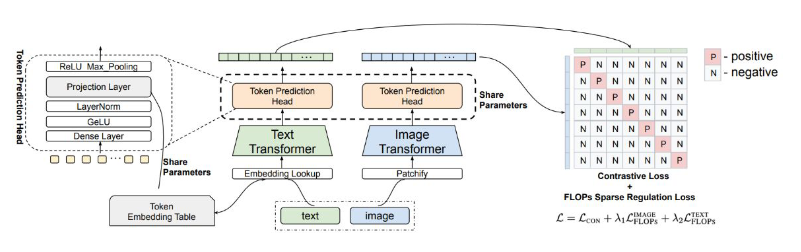
\includegraphics[width=1\linewidth]{tikz/STAIR.png}
    \caption{An example of STAIR}
    \label{fig:STAIR}
\end{figure}


Results showed that if we take the top 20 tokens predicted by STAIR for an image, and plot them with font size indicates prediction weight, we could see the relevance of each word in the embedding space.

\begin{figure}[H]
    \centering
    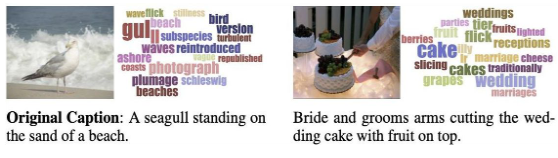
\includegraphics[width=1\linewidth]{tikz/STAIR Results.png}
    \caption{STAIR Results}
    \label{fig:STAIR-Results}
\end{figure}



\subsubsection{Objective Functions: fine-grained supervision}

An example that belongs to this improvement category is FILIP. 

The idea is that, instead of modeling cross-modal interaction via only the global features of the entire image and text sequence such as in CLIP, the fine-grained interaction between image
patches and textual tokens is taken into account.

The architecture still uses dual encoders:
\begin{itemize}
    \item \textbf{Visual encoder}: For the visual modality, the image encoder is ViT.
    \vspace{5 pt}
    \item \textbf{Text Encoder}: For the textual modality, after the word embedding layer, the token embeddings are fed into a \textbf{decoder-only Transformer}.
\end{itemize}

On top of the image and text encoders, the
representations are linearly projected to the
multi-modal common space.

\begin{figure}[H]
    \centering
    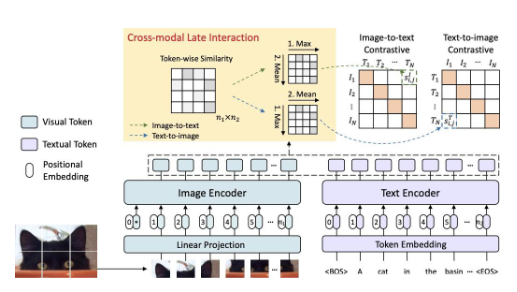
\includegraphics[width=1\linewidth]{tikz/FILIP.png}
    \caption{An example of FILIP}
    \label{fig:FILIP}
\end{figure}

The finer-level alignment is achieved through a \textbf{cross-modal late interaction
mechanism}: first compute the token-wise similarity, then aggregate the matrix by max pooling, then compute the contrastive loss.



At the end, the network will learn word-patch alignment that is good for visualization.

The image below shows an example with the class label "balloon" (5) which is fed into the prompt “[BOS] a photo of a balloon. [EOS]” and tokenized into  8 token sequence. The model will learn corresponding tokens that activate in patches where the class is seen. The location index of the class label “balloon” inside the patches is “5”.

\begin{figure}[H]
    \centering
    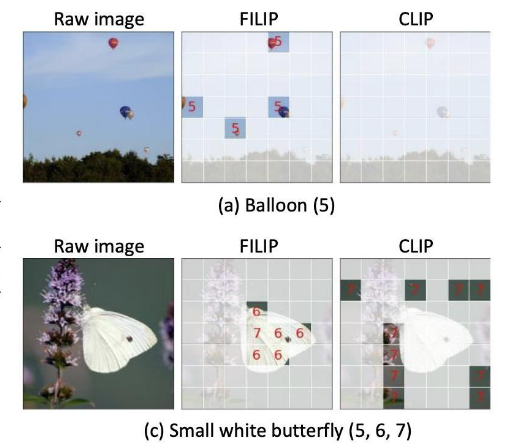
\includegraphics[width=1\linewidth]{tikz/FILIP visualization.png}
    \caption{An example of word-patch visualization with FILIP}
    \label{fig:FILIP-visualization}
\end{figure}



\subsubsection{Objective Functions: adding a generative branch}

Clip trains an image encoder and text encoder with a constrastive loss. CoCa (Constrastive Captioner) reinforces the learning by adding a generative branch for text trained with extra loss term, \textbf{captionin loss}. Basically, CoCa improved Clip by pushing it to perform an extra task, captioning task.


This allowed to obtain a  pre-train image-text encoder-decoder foundation model, trained using jointly a contrastive loss and captioning loss. Thus, the model is not limited in  just visual recognition task, but also to perform downstream tasks including image-captioning, vision-language alignment, ecc...

As can be seen in the image below, CoCa unifies a three models into one: single-encoder, dual-encoder, and encoder-decoder paradigms. It is a \textbf{ image-text foundation model with the capabilities of all three approaches}.

\begin{figure}[H]
    \centering
    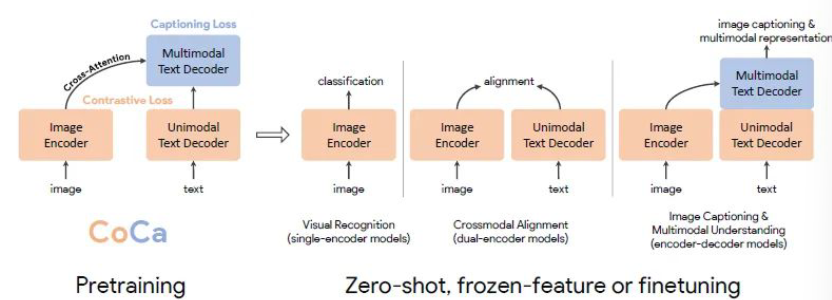
\includegraphics[width=1\linewidth]{tikz/CoCa.png}
    \caption{CoCa}
    \label{fig:CoCa}
\end{figure}

From the architecture prospective:

\begin{itemize}
    \item Cross-attention is omitted in unimodal decoder layer, thus it just encodes text-only representations.

    \vspace{ 5 pt}
    \item The Multimodal decoder cross-attending to image encoder outputs to learn multimodal representations.
    \vspace{5 pt}
    \item  Training is performed mixing image-text and image-label (JFT-3B) data for pre-training.

    \vspace{5pt}
    \item The loss used for the dual encoder is  the contrastive loss (same as CLIP).

    \vspace{5 pt}
    \item To train the captioner, an additional generative branch is added. While the dual-encoder approach encodes the text as a whole, the generative approach (captioner) aims for detailed granularity and requires the model to
predict the exact tokenized texts of $y$.

\end{itemize}

This is done \textbf{autoregressively}, by using the following formula:



$$L_{Cap} = - \sum_{t=1}^{T}\log P_{\theta}(y_t|y_{<t},x) $$

The loss reflects one tipical way to generate a text $y$ using the probability of generating a token $y_t$ given all the previous predictions and the visual information $x$ (coming from the image encoder). This training approach is also defined as \textbf{autoregressive learning}. The loss maximizes the
conditional likelihood ($\theta$) of the paired text-images $y<t,x$ under the forward autoregressive factorization.

\subsubsection{SIMVLM}

SIMVLM is a variation of CoCa, actually was the first attempt made by the same authors of CoCa that however was not competitive with CLIP.

The architecture employs a transformer Encoder-Decoder. The idea is to ask the model to predict autoregressively the next token given as input some visual and text token embeddings.

\begin{figure}[H]
    \centering
    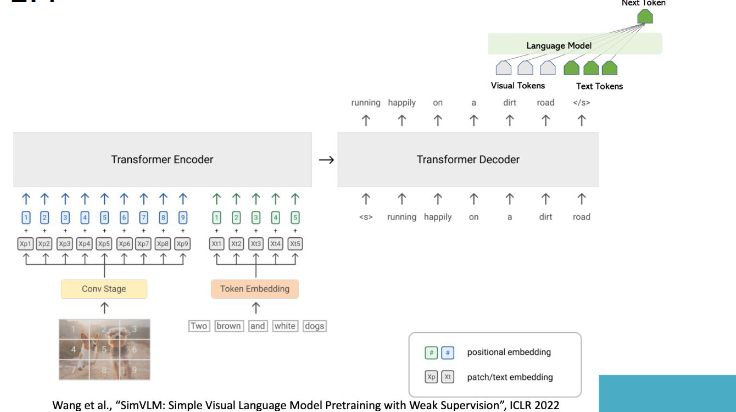
\includegraphics[width=1\linewidth]{tikz/SIMVLM.png}
    \caption{An example of SIMVLM}
    \label{fig:SIMVLM}
\end{figure}

At the end, what we as seen so far is how to takle Vision-Language model in three different designs: Dual encoders (CLIP) but text cannot be generated, Encoder-decoder (SIMVLM) where text can be generated but it is not competitive in respect to CLIP, Fusion decoder (Coca) which takes both advantages.


\begin{figure}[H]
    \centering
    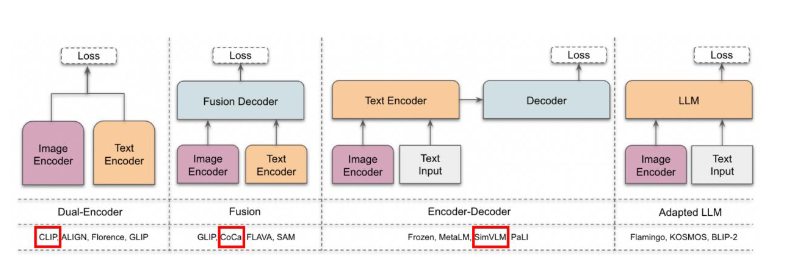
\includegraphics[width=1\linewidth]{tikz/CLIP Recap.png}
    \caption{CLIP architectures recap}
    \label{fig:CLIP-recap}
\end{figure}

CLIP learns good representations but cannot generate. Coca has a fusion decoder which digest multimodel information with cross-attention inside becoming a strong obtag that can generate text. SimVim can generate but uses not a proper loss thus is not competitive. \textbf{FLAMINGO} blends the two encoders with an additional LLM.

\section{LLMs as Universal Interface}

Multimodal systems can provide a more flexible way of interaction to provide the input needed by the model: for example typing (text), talking (audio), or pointing your camera at something can be used throughout the question.

How can we utilize the potentials of LLMs for creating a general-purpose assistant? So far (GPT3), the interface had limited interactivity and adaptability to the user’s
instructions. They must be able to ingest a \textbf{multimodal prompt},  containing images and/or videos interleaved with text.

The idea is to equip LLMs with eyes to see the world by training them on vision-conditioned language generation tasks and so use LLMs as a general interface for other modalities and thus make use of facts that it has learned during language-only pre-training

The model is finetuned on instruction-following and use task instructions to
repurpose the model.

\subsection{Frozen LM Prefix}

This model contains Frozen Visual encoder,  NF-ResNet50, language embeddings and language model to produce texts.

\textbf{Forzen}: the visual and text modalities are incorporated as input without needing to update the encoder's weights. 

Concatenated textual and visual embeddings are fed to the decoder of the LLM, which generates a textual output autoregressively.

\begin{figure}[H]
    \centering
    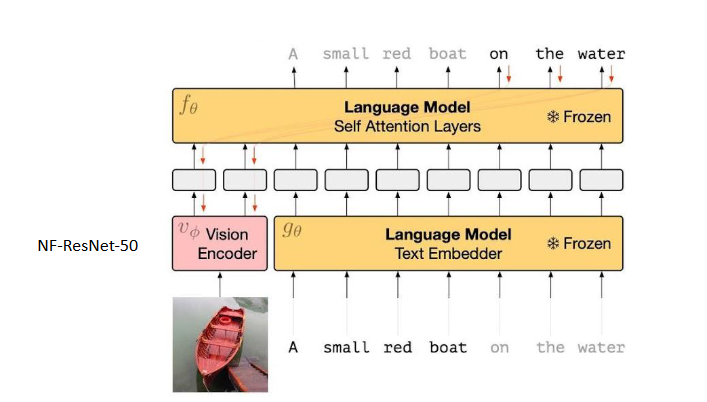
\includegraphics[width=1\linewidth]{tikz/Flamingo 1.png}
    \caption{An example of Frozen architecture}
    \label{fig:Frozen}
\end{figure}

Subsequently, finetune the image encoder to improve the quality of its representations. Still, its outputs are directly used as soft prompts for the LLM. 

\textbf{soft prompt}: is a technique where a numerical representation is used to guide the behavior of the language model without directly modifying its weights. It is like giving a suggestion or a guide to the model on what it should focus on. In practice, the information extracted from the image guides the language model in generating text, answering questions, or performing other linguistic tasks.



\begin{figure}[H]
    \centering
    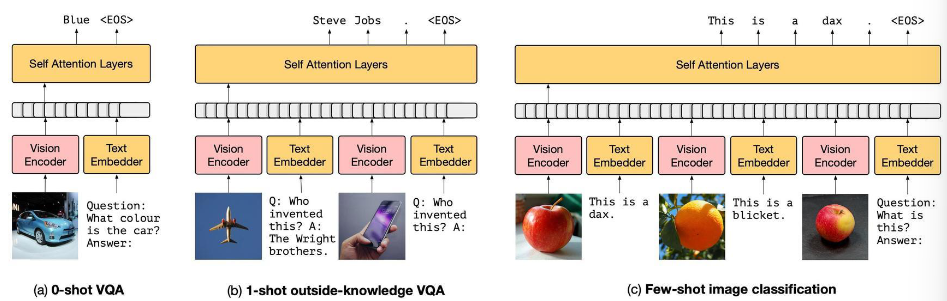
\includegraphics[width=1\linewidth]{tikz/Flaming 2.png}
    \caption{An example of finetuning Frozen}
    \label{fig:Frozen-finetune}
\end{figure}


\subsection{Flamingo}
Flamingo improved the Frozen design. It bridges powerful pretrained vision-only encoder and language-only models by using novel architecture components.

The model can digest image, video and text. Thus,  it can perform different tasks such as classification, captioning, or question-answering, completion task.

The vision models are trained in CLIP like fashion and are needed to “perceive” visual scenes. The LLMs are needed to perform a basic form of reasoning.

The novelty component are \textbf{Perceiver resampler} and \textbf{Gated XATTN-DENSE}, which are trained from scratch.


\begin{figure}[H]
    \centering
    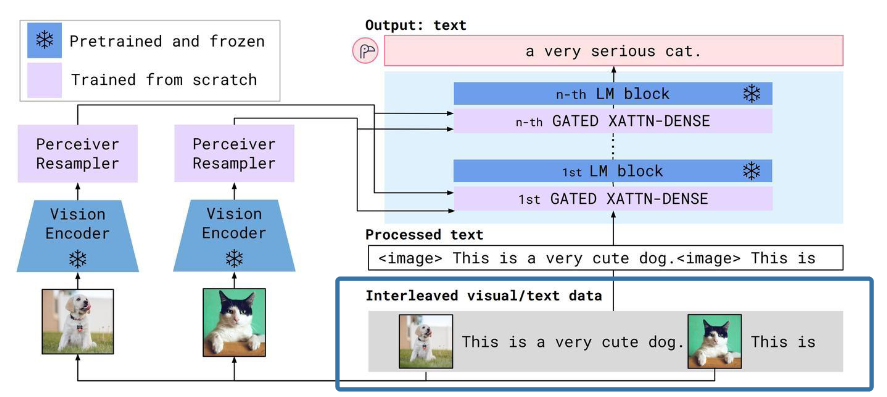
\includegraphics[width=1\linewidth]{tikz/Flamingo 3.png}
    \caption{Flamingo}
    \label{fig:Flamingo}
\end{figure}

The model is trained with sequences of arbitrarily interleaved visual and textual data input. The output is free form text.

\begin{figure}[H]
    \centering
    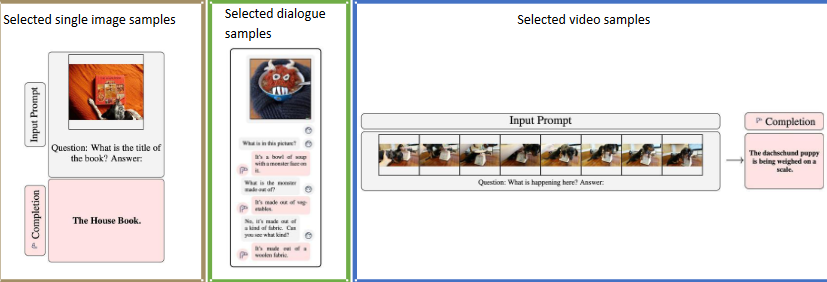
\includegraphics[width=1\linewidth]{tikz/Falingo input-output.png}
    \caption{Flamingo input/output}
    \label{fig:Flaming input/output}
\end{figure}

\begin{figure}[H]
    \centering
    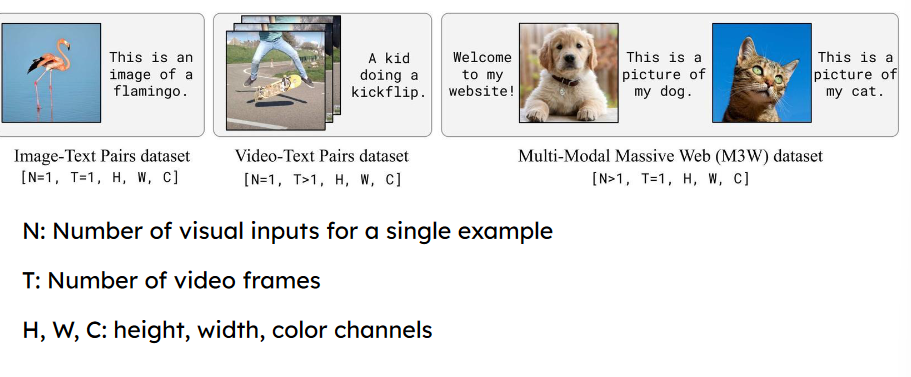
\includegraphics[width=1\linewidth]{tikz/Flamingo Input.png}
    \caption{Flamingo input}
    \label{fig:Flamingo-input}
\end{figure}

One first challenge here is that the visual input can be of arbitrary dimension, thus goal of the perceiver is to handle them in a smarter way, obtaining a meaninfull representation and fixed dimension.  Due to its flexibility, it can be trained on large-scale multimodal web. 

XATTN try to merge information coming from images with those coming from text. XATTN are Gated and Dense.

\subsubsection{Vision and Text Encoder}

The 2 Vision encoders are pretrained and frozen  Normalizer Free ResNet (NFNet), which are models trained with a CLIP-like procedure (contrastive learning) using 2 dataset of paired image, text information, totaling 2.1M (image, text) pairs. This is 5x larger than the dataset CLIP was trained on.

For the text encoder, used only to train the vision encoder in CLIP manner, is BERT instead of GPT-2.

Text and vision embeddings are meanpooled before being projected to the joint embedding space.

\subsubsection{Language Model}

Flamingo uses \textbf{Chinchilla} as their language model. To be able to generate text conditioned on both text and visual inputs, Flamingo relied on Perceiver Resampler and GATED XATTN-DENSE layers.

\textbf{Perceiver Resampler}

The perceiver resampler module maps a variable size gird of spatio-temporal visual features output by the Vision Encoder to a fixed number of output tokens (in the figure \ref{fig:Perceiver-resampler}, 5), independently from the input image resolution or the number of input video framas. This transformer has a set of learned latent vectors as queries, and the key and values are a concatenation of the spatio-temporal visual features with time embeddings, which are then flattened.

Specifically, only this set of latent queries (5) are learnt during training. The output representation of the module will be subsequently used in the XATT module.


\begin{figure}[H]
    \centering
    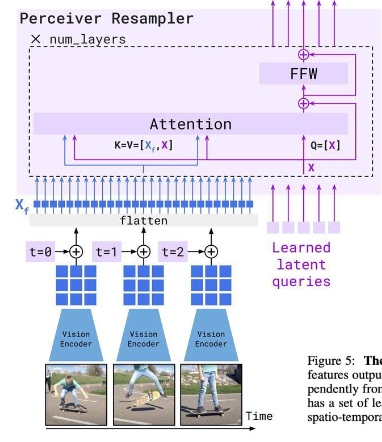
\includegraphics[width=1\linewidth]{tikz/Perceiver Resampler.png}
    \caption{An example of Perceiver Resampler}
    \label{fig:Perceiver-resampler}
\end{figure}

\textbf{Gated XATTN-Dense layers}

GATED XATTN-DENSE layers are inserted between existing pretrained and frozen LM layers to allow the LM to attend more efficiently to the visual tokens when generating text tokens.

The keys and values in these layers are obtained from the vision features while the queries are derived from the language inputs. They are followed by dense FF layers. These layers are gated (tanh gate) so that the LM is kept intact at initialization for improved stability and performance.

The output of Gated XATTN-Dense layers is used as key, value, query of the LM layer.

\begin{figure}[H]
    \centering
    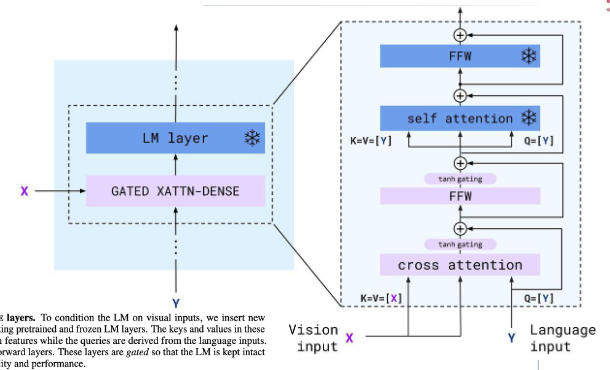
\includegraphics[width=1\linewidth]{tikz/Gated XATTN-Dense layers.png}
    \caption{An example of Gated XATTN-Dense layers}
    \label{fig:Gated-XATTN-Dense-layers}
\end{figure}

\textbf{Autoregressive learning}

Then, the output is predicted in an autoregressive approach. The image below shows the flow: first, input is taken. Image tag is processed by adding special tokens in order to obtain the preprocessed text used as query of the Masked Cross Attention. Also, the image is passed to the visual encoders; Then, key and value of the masked cross attention are retrieved from perceiver Resamplers; Subsequently, Masked cross attention is computed in orderd to predict the textual output. This is then used to processed text to predict a new textual output until the special stopping token "EOC" is predicted.


\begin{figure}[H]
    \centering
    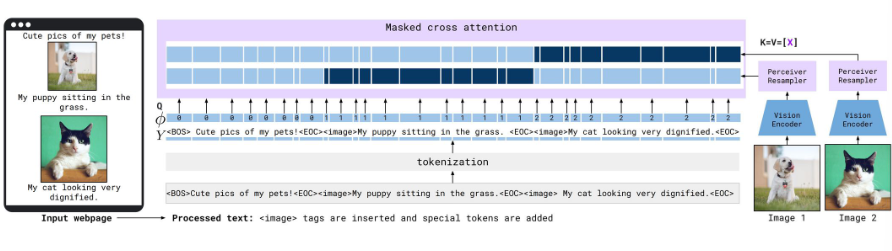
\includegraphics[width=1\linewidth]{Flamingo Autoregressive.png}
    \caption{Enter Caption}
    \label{fig:enter-label}
\end{figure}

\subsubsection{summary}

Flamingo unifies a strong single-modal models by connectors: it joints LM (Chincilla, from deep mind) and Vision encoderd (ResNet) by using Perceiver-based architecture, with a fixed number of visual tokens to support images and videos, and Interleave cross-attention layers with language only self-attention layers.

Heterogeneous training data:  Combine web scraping with existing image-text or video text datasets.



\begin{figure}[H]
    \centering
    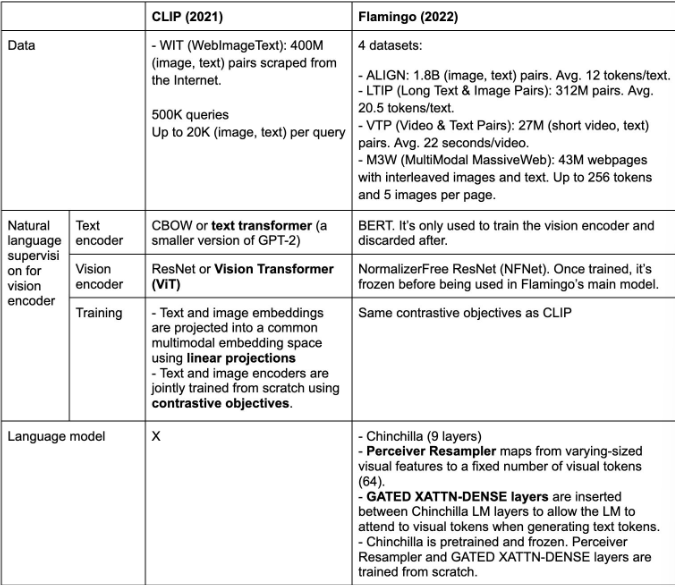
\includegraphics[width=1\linewidth]{tikz/Clip vs Flamingo.png}
    \caption{The image shows a comparison between Clip and Flamingo.}
    \label{fig:enter-label}
\end{figure}








